\documentclass[10pt,a4paper]{amsart}
\usepackage[margin=19mm]{geometry}
\usepackage{amsmath,amssymb,mathtools}
\usepackage[scr=rsfs,cal=euler]{mathalfa}
\usepackage{xfrac}
\usepackage[unicode,hidelinks,bookmarks=false]{hyperref}
\newcommand{\ie}{i.e.\ }
\newcommand{\cf}{cf.\ }
\newcommand{\resp}{respectively\ }
\newcommand{\Subsection}{\subsection}
\providecommand{\nobreakdash}{\nobreak\hbox{-}}
\setlength{\emergencystretch}{2em}
\multlinegap0pt
\usepackage{tikz}
\usepackage{amssymb}
\usepackage{float}
\newtheorem{lemma}{Lemma}
\newcommand{\diam}{\operatorname{diam}}		
\newcommand{\mc}{\mathcal}
\newcommand{\spine}{\operatorname{Spine}}
\title{Continuum-wise hyperbolicity is exactly the pseudo-Anosov dynamics with spine singularities}
\author{Rodrigo Arruda, Bernardo Carvalho, Piotr Oprocha, Alberto Sarmiento}
\date{Source: arXiv:2606.11943v1 (CC BY 4.0)}
\begin{document}
\maketitle

\noindent\emph{Source and licence.} Continuum-wise hyperbolicity is exactly the pseudo-Anosov dynamics with spine singularities. Version arXiv:2606.11943v1 (CC BY 4.0), distributed by arXiv under the Creative Commons Attribution 4.0 International licence, http://creativecommons.org/licenses/by/4.0/, as recorded in the arXiv licence metadata for this exact version and shown on the abstract page https://arxiv.org/abs/2606.11943v1. Full licence notice: \texttt{licenses/arxiv-2606.11943-CC-BY-4.0.txt}.\par\smallskip

\noindent\textit{Editorial scope.} Counted unit: the article's lemma lem:drho (source0.tex lines 655--660). The article's complete original proof of it is delivered with it (source0.tex lines 662--804, one \texttt{proof} environment of 143 lines). No mathematics is written, repaired or re-derived: the statement and the proof are the article's own lines, in the article's own notation, and no retained line is substituted or re-flowed.  No further source-local context is needed: every cross-reference of every retained line resolves inside the two delivered spans.  Nothing was omitted from any retained span, so the package carries no omission record.  No retained line contains a citation, so the wrapper carries no bibliography and no bibliography entry.  The retained lines contain the article's own diagram code, which the wrapper typesets with the standard tikz packages; no image file is delivered and the package declares no asset dependency.  Editorial formatting only, in addition: an AMS \texttt{amsart} preamble that restates the article's own declarations and macros used by the retained lines, namely the environments \texttt{lemma} on separate counters, together with the standard packages those lines need.  The retained environments print in this document as Lemma 1 in order of appearance, whereas the article prints the same items with the numbering of its own full document.  The complete native source of the article as distributed in the arXiv e-print for this exact version is bundled unchanged as \texttt{sources/202586/source0.tex}.
\begin{lemma}\label{lem:drho}
The function $d_\rho$ is a metric uniformly equivalent to $d$. 
Furthermore, for each $x\in S\setminus \spine(f)$, there is an open set $U_x$ such that if
$I\subset \mc{F}^s\cap U_x$ $($resp. $I\subset \mc{F}^u\cap U_x)$ 
then $\diam_{d_\rho}(I)= \mu^u(I)$ $($resp. $\diam_{d_\rho}(I)=\mu^s(I))$.
\end{lemma}

\begin{proof}
It is clear that $d_\rho$ satisfies the triangle inequality since the union of two rectifiable arcs is a rectifiable arc itself. Also, since in $D_i$ we have concrete coordinates, it is clear that there is a finite set of arcs either in $\mc{F}^s$ or $\mc{F}^u$, such that any arc $\gamma$ connecting $x,y$ must have a subset isotopic to one of them. This implies that $d_\rho(x,y)>0$ for $x\neq y$. So indeed, $d_\rho$ is a metric. We can use topological rectangles in $\mc{D}_1$ or $\mc{D}_2$ to show that any open set in $d$ contains a ball in $d_\rho$ and vice-versa (see Figure~\ref{fig:sketch}). Then $d$ and $d_\rho$ define the same topology, and so are uniformly equivalent as $S$ is compact.

\begin{figure}[ht]
\centering
\resizebox{0.40\linewidth}{!}{%
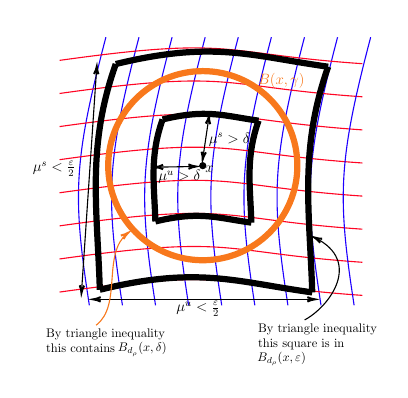
\begin{tikzpicture}[x=0.24pt,y=0.24pt,yscale=-1,xscale=1]
\useasboundingbox (53,0) rectangle (583,515);

\draw [color={rgb, 255:red, 30; green, 0; blue, 255 }  ,draw opacity=1 ]   (170.76,14.37) .. controls (120.93,203.73) and (120.93,256.05) .. (145.85,418) ;
\draw [color={rgb, 255:red, 30; green, 0; blue, 255 }  ,draw opacity=1 ]   (220.59,14.37) .. controls (170.76,203.73) and (170.76,256.05) .. (195.68,418) ;
\draw [color={rgb, 255:red, 30; green, 0; blue, 255 }  ,draw opacity=1 ]   (270.42,14.37) .. controls (220.59,203.73) and (220.59,256.05) .. (245.51,418) ;
\draw [color={rgb, 255:red, 30; green, 0; blue, 255 }  ,draw opacity=1 ]   (320.25,14.37) .. controls (270.42,203.73) and (270.42,256.05) .. (295.34,418) ;
\draw [color={rgb, 255:red, 30; green, 0; blue, 255 }  ,draw opacity=1 ]   (370.09,14.37) .. controls (320.25,203.73) and (320.25,256.05) .. (345.17,418) ;
\draw [color={rgb, 255:red, 30; green, 0; blue, 255 }  ,draw opacity=1 ]   (419.92,14.37) .. controls (370.09,203.73) and (370.09,256.05) .. (395,418) ;
\draw [color={rgb, 255:red, 30; green, 0; blue, 255 }  ,draw opacity=1 ]   (469.75,14.37) .. controls (419.92,203.73) and (419.92,256.05) .. (444.83,418) ;
\draw [color={rgb, 255:red, 30; green, 0; blue, 255 }  ,draw opacity=1 ]   (519.58,14.37) .. controls (469.75,203.73) and (469.75,256.05) .. (494.66,418) ;
\draw [color={rgb, 255:red, 255; green, 5; blue, 36 }  ,draw opacity=1 ]   (101,49.25) .. controls (367.59,11.88) and (340.19,39.29) .. (556.95,54.24) ;
\draw [color={rgb, 255:red, 255; green, 5; blue, 36 }  ,draw opacity=1 ]   (101,99.08) .. controls (367.59,61.71) and (340.19,89.12) .. (556.95,104.07) ;
\draw [color={rgb, 255:red, 255; green, 5; blue, 36 }  ,draw opacity=1 ]   (101,148.91) .. controls (367.59,111.54) and (340.19,138.95) .. (556.95,153.9) ;
\draw [color={rgb, 255:red, 255; green, 5; blue, 36 }  ,draw opacity=1 ]   (101,198.75) .. controls (367.59,161.37) and (340.19,188.78) .. (556.95,203.73) ;
\draw [color={rgb, 255:red, 255; green, 5; blue, 36 }  ,draw opacity=1 ]   (101,248.58) .. controls (367.59,211.2) and (340.19,238.61) .. (556.95,253.56) ;
\draw [color={rgb, 255:red, 255; green, 5; blue, 36 }  ,draw opacity=1 ]   (101,298.41) .. controls (367.59,261.03) and (340.19,288.44) .. (556.95,303.39) ;
\draw [color={rgb, 255:red, 255; green, 5; blue, 36 }  ,draw opacity=1 ]   (101,348.24) .. controls (367.59,310.86) and (340.19,338.27) .. (556.95,353.22) ;
\draw [color={rgb, 255:red, 255; green, 5; blue, 36 }  ,draw opacity=1 ]   (101,398.07) .. controls (367.59,360.69) and (340.19,388.1) .. (556.95,403.05) ;
\draw [color={rgb, 255:red, 30; green, 0; blue, 255 }  ,draw opacity=1 ]   (569.41,14.37) .. controls (519.58,203.73) and (519.58,256.05) .. (544.49,418) ;
\draw  [fill={rgb, 255:red, 0; green, 0; blue, 0 }  ,fill opacity=1 ] (321.15,207.75) .. controls (321.15,205.26) and (319.13,203.24) .. (316.64,203.24) .. controls (314.14,203.24) and (312.12,205.26) .. (312.12,207.75) .. controls (312.12,210.25) and (314.14,212.27) .. (316.64,212.27) .. controls (319.13,212.27) and (321.15,210.25) .. (321.15,207.75) -- cycle ;
\draw [color={rgb, 255:red, 0; green, 0; blue, 0 }  ,draw opacity=1 ][line width=2.25]    (256.12,138.21) .. controls (236.25,194.2) and (243.48,235.75) .. (245.29,291.75) ;
\draw [color={rgb, 255:red, 0; green, 0; blue, 0 }  ,draw opacity=1 ][line width=2.25]    (400.63,140.01) .. controls (380.76,196.01) and (387.99,237.56) .. (389.79,293.55) ;
\draw [color={rgb, 255:red, 0; green, 0; blue, 0 }  ,draw opacity=1 ][line width=2.25]    (256.12,138.21) .. controls (322.96,121.95) and (348.25,132.79) .. (400.63,140.01) ;
\draw [color={rgb, 255:red, 0; green, 0; blue, 0 }  ,draw opacity=1 ][line width=2.25]    (245.29,291.75) .. controls (312.12,275.49) and (337.41,286.33) .. (389.79,293.55) ;
\draw    (325.71,135.98) -- (316.79,196.02) ;
\draw [shift={(316.5,198)}, rotate = 278.44] [color={rgb, 255:red, 0; green, 0; blue, 0 }  ][line width=0.75]    (10.93,-3.29) .. controls (6.95,-1.4) and (3.31,-0.3) .. (0,0) .. controls (3.31,0.3) and (6.95,1.4) .. (10.93,3.29)   ;
\draw [shift={(326,134)}, rotate = 98.44] [color={rgb, 255:red, 0; green, 0; blue, 0 }  ][line width=0.75]    (10.93,-3.29) .. controls (6.95,-1.4) and (3.31,-0.3) .. (0,0) .. controls (3.31,0.3) and (6.95,1.4) .. (10.93,3.29)   ;
\draw    (248,209.97) -- (304,209.03) ;
\draw [shift={(306,209)}, rotate = 179.05] [color={rgb, 255:red, 0; green, 0; blue, 0 }  ][line width=0.75]    (10.93,-3.29) .. controls (6.95,-1.4) and (3.31,-0.3) .. (0,0) .. controls (3.31,0.3) and (6.95,1.4) .. (10.93,3.29)   ;
\draw [shift={(246,210)}, rotate = 359.05] [color={rgb, 255:red, 0; green, 0; blue, 0 }  ][line width=0.75]    (10.93,-3.29) .. controls (6.95,-1.4) and (3.31,-0.3) .. (0,0) .. controls (3.31,0.3) and (6.95,1.4) .. (10.93,3.29)   ;
\draw  [color={rgb, 255:red, 248; green, 120; blue, 28 }  ,draw opacity=1 ][line width=2.25]  (174.26,207.75) .. controls (174.26,129.12) and (238,65.38) .. (316.64,65.38) .. controls (395.27,65.38) and (459.01,129.12) .. (459.01,207.75) .. controls (459.01,286.38) and (395.27,350.13) .. (316.64,350.13) .. controls (238,350.13) and (174.26,286.38) .. (174.26,207.75) -- cycle ;
\draw [color={rgb, 255:red, 0; green, 0; blue, 0 }  ,draw opacity=1 ][line width=2.25]    (185.63,54.77) .. controls (141.66,178.69) and (157.65,270.63) .. (161.64,394.56) ;
\draw [color={rgb, 255:red, 0; green, 0; blue, 0 }  ,draw opacity=1 ][line width=2.25]    (505.43,58.77) .. controls (461.46,182.69) and (477.45,274.63) .. (481.44,398.55) ;
\draw [color={rgb, 255:red, 0; green, 0; blue, 0 }  ,draw opacity=1 ][line width=2.25]    (185.63,54.77) .. controls (333.54,18.79) and (389.5,42.78) .. (505.43,58.77) ;
\draw [color={rgb, 255:red, 0; green, 0; blue, 0 }  ,draw opacity=1 ][line width=2.25]    (161.64,394.56) .. controls (309.55,358.58) and (365.52,382.56) .. (481.44,398.55) ;
\draw    (156.87,61) -- (134.13,397) ;
\draw [shift={(134,399)}, rotate = 273.87] [color={rgb, 255:red, 0; green, 0; blue, 0 }  ][line width=0.75]    (10.93,-3.29) .. controls (6.95,-1.4) and (3.31,-0.3) .. (0,0) .. controls (3.31,0.3) and (6.95,1.4) .. (10.93,3.29)   ;
\draw [shift={(157,59)}, rotate = 93.87] [color={rgb, 255:red, 0; green, 0; blue, 0 }  ][line width=0.75]    (10.93,-3.29) .. controls (6.95,-1.4) and (3.31,-0.3) .. (0,0) .. controls (3.31,0.3) and (6.95,1.4) .. (10.93,3.29)   ;
\draw    (483,409) -- (154,409) ;
\draw [shift={(152,409)}, rotate = 360] [color={rgb, 255:red, 0; green, 0; blue, 0 }  ][line width=0.75]    (10.93,-3.29) .. controls (6.95,-1.4) and (3.31,-0.3) .. (0,0) .. controls (3.31,0.3) and (6.95,1.4) .. (10.93,3.29)   ;
\draw [shift={(485,409)}, rotate = 180] [color={rgb, 255:red, 0; green, 0; blue, 0 }  ][line width=0.75]    (10.93,-3.29) .. controls (6.95,-1.4) and (3.31,-0.3) .. (0,0) .. controls (3.31,0.3) and (6.95,1.4) .. (10.93,3.29)   ;
\draw    (470,440) .. controls (508.81,419.1) and (556.52,351.68) .. (486.07,316.53) ;
\draw [shift={(485,316)}, rotate = 25.92] [color={rgb, 255:red, 0; green, 0; blue, 0 }  ][line width=0.75]    (10.93,-3.29) .. controls (6.95,-1.4) and (3.31,-0.3) .. (0,0) .. controls (3.31,0.3) and (6.95,1.4) .. (10.93,3.29)   ;
\draw [color={rgb, 255:red, 248; green, 120; blue, 28 }  ,draw opacity=1 ]   (156,448) .. controls (195.6,418.3) and (164.63,340.58) .. (202.82,309.91) ;
\draw [shift={(204,309)}, rotate = 143.13] [color={rgb, 255:red, 248; green, 120; blue, 28 }  ,draw opacity=1 ][line width=0.75]    (10.93,-3.29) .. controls (6.95,-1.4) and (3.31,-0.3) .. (0,0) .. controls (3.31,0.3) and (6.95,1.4) .. (10.93,3.29)   ;

\draw (318.64,206.64) node [anchor=north west][inner sep=0.75pt]  [font=\large,xscale=0.45,yscale=0.45]  {$x$};
\draw (324,156.4) node [anchor=north west][inner sep=0.75pt]  [font=\large,xscale=0.45,yscale=0.45]  {$\mu ^{s}  >\delta $};
\draw (248,213.4) node [anchor=north west][inner sep=0.75pt]  [font=\large,xscale=0.45,yscale=0.45]  {$\mu ^{u}  >\delta $};
\draw (59,199.4) node [anchor=north west][inner sep=0.75pt]  [font=\large,xscale=0.45,yscale=0.45]  {$\mu ^{s} < \frac{\varepsilon }{2}$};
\draw (275,410.4) node [anchor=north west][inner sep=0.75pt]  [font=\large,xscale=0.45,yscale=0.45]  {$\mu ^{u} < \frac{\varepsilon }{2}$};
\draw (398,444) node [anchor=north west][inner sep=0.75pt]  [xscale=0.45,yscale=0.45] [align=left] {By triangle inequality\\this square is in};
\draw (397,486.4) node [anchor=north west][inner sep=0.75pt]  [xscale=0.45,yscale=0.45]  {$B_{d_{\rho}}( x,\varepsilon )$};
\draw (79,452) node [anchor=north west][inner sep=0.75pt]  [xscale=0.45,yscale=0.45] [align=left] {By triangle inequality\\this contains};
\draw (187,472.4) node [anchor=north west][inner sep=0.75pt]  [xscale=0.45,yscale=0.45]  {$B_{d_{\rho}}( x,\delta )$};
\draw (398,66.4) node [anchor=north west][inner sep=0.75pt]  [font=\large,color={rgb, 255:red, 248; green, 120; blue, 28 }  ,opacity=1 ,xscale=0.45,yscale=0.45]  {$B( x,\gamma )$};

\end{tikzpicture}
}
\hfill
\resizebox{0.49\linewidth}{!}{%
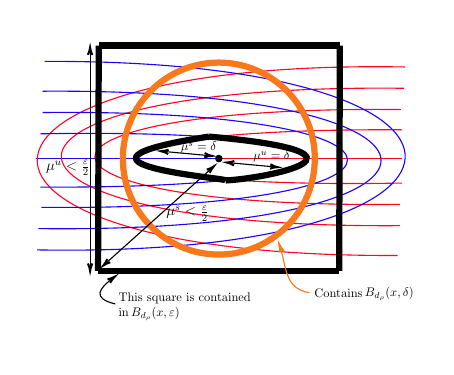
\begin{tikzpicture}[x=0.24pt,y=0.24pt,yscale=-1,xscale=1]
\useasboundingbox (40,0) rectangle (640,480);
\draw [color={rgb, 255:red, 30; green, 0; blue, 255 }  ,draw opacity=1 ]   (52,197.06) -- (327.79,197.06) ;
\draw [color={rgb, 255:red, 255; green, 5; blue, 36 }  ,draw opacity=1 ]   (327.79,197.06) -- (603.58,197.06) ;
\draw  [fill={rgb, 255:red, 0; green, 0; blue, 0 }  ,fill opacity=1 ] (332.6,197.06) .. controls (332.6,194.41) and (330.45,192.25) .. (327.79,192.25) .. controls (325.13,192.25) and (322.98,194.41) .. (322.98,197.06) .. controls (322.98,199.72) and (325.13,201.87) .. (327.79,201.87) .. controls (330.45,201.87) and (332.6,199.72) .. (332.6,197.06) -- cycle ;
\draw [color={rgb, 255:red, 255; green, 5; blue, 36 }  ,draw opacity=1 ]   (603.58,233.94) .. controls (63.22,243.56) and (72.84,150.56) .. (603.58,153.77) ;
\draw [color={rgb, 255:red, 255; green, 5; blue, 36 }  ,draw opacity=1 ]   (600.37,266.01) .. controls (-10.53,272.42) and (-13.74,116.89) .. (601.98,123.3) ;
\draw [color={rgb, 255:red, 255; green, 5; blue, 36 }  ,draw opacity=1 ]   (600.37,298.08) .. controls (-79.48,302.89) and (-81.08,83.22) .. (606.79,91.24) ;
\draw [color={rgb, 255:red, 255; green, 5; blue, 36 }  ,draw opacity=1 ]   (597.17,342.97) .. controls (-138.81,346.18) and (-117.96,46.34) .. (608.39,59.17) ;
\draw [color={rgb, 255:red, 30; green, 0; blue, 255 }  ,draw opacity=1 ]   (59.15,159.81) .. controls (599.5,150.19) and (589.88,243.19) .. (59.15,239.98) ;
\draw [color={rgb, 255:red, 30; green, 0; blue, 255 }  ,draw opacity=1 ]   (62.36,127.74) .. controls (673.26,121.33) and (676.47,276.86) .. (60.75,270.45) ;
\draw [color={rgb, 255:red, 30; green, 0; blue, 255 }  ,draw opacity=1 ]   (62.36,95.67) .. controls (742.21,90.86) and (743.81,310.53) .. (55.94,302.51) ;
\draw [color={rgb, 255:red, 30; green, 0; blue, 255 }  ,draw opacity=1 ]   (65.56,50.78) .. controls (801.54,47.57) and (780.69,347.41) .. (54.34,334.58) ;
\draw [line width=2.25]    (338,230) .. controls (348,227) and (47,205) .. (313,164) ;
\draw [line width=2.25]    (338,230) .. controls (399,227) and (593,189) .. (313,164) ;
\draw    (242.99,186.18) -- (315.01,192.82) ;
\draw [shift={(317,193)}, rotate = 185.26] [color={rgb, 255:red, 0; green, 0; blue, 0 }  ][line width=0.75]    (10.93,-3.29) .. controls (6.95,-1.4) and (3.31,-0.3) .. (0,0) .. controls (3.31,0.3) and (6.95,1.4) .. (10.93,3.29)   ;
\draw [shift={(241,186)}, rotate = 5.26] [color={rgb, 255:red, 0; green, 0; blue, 0 }  ][line width=0.75]    (10.93,-3.29) .. controls (6.95,-1.4) and (3.31,-0.3) .. (0,0) .. controls (3.31,0.3) and (6.95,1.4) .. (10.93,3.29)   ;
\draw    (341.99,203.18) -- (414.01,209.82) ;
\draw [shift={(416,210)}, rotate = 185.26] [color={rgb, 255:red, 0; green, 0; blue, 0 }  ][line width=0.75]    (10.93,-3.29) .. controls (6.95,-1.4) and (3.31,-0.3) .. (0,0) .. controls (3.31,0.3) and (6.95,1.4) .. (10.93,3.29)   ;
\draw [shift={(340,203)}, rotate = 5.26] [color={rgb, 255:red, 0; green, 0; blue, 0 }  ][line width=0.75]    (10.93,-3.29) .. controls (6.95,-1.4) and (3.31,-0.3) .. (0,0) .. controls (3.31,0.3) and (6.95,1.4) .. (10.93,3.29)   ;
\draw  [color={rgb, 255:red, 248; green, 120; blue, 28 }  ,draw opacity=1 ][line width=2.25]  (183.29,197.06) .. controls (183.29,117.26) and (247.98,52.56) .. (327.79,52.56) .. controls (407.59,52.56) and (472.29,117.26) .. (472.29,197.06) .. controls (472.29,276.87) and (407.59,341.56) .. (327.79,341.56) .. controls (247.98,341.56) and (183.29,276.87) .. (183.29,197.06) -- cycle ;
\draw [line width=2.25]    (147,27) -- (146,366) ;
\draw [line width=2.25]    (509,366) -- (146,366) ;
\draw [line width=2.25]    (510,27) -- (147,27) ;
\draw [line width=2.25]    (510,27) -- (509,366) ;
\draw    (155.49,356.66) -- (318.51,210.34) ;
\draw [shift={(320,209)}, rotate = 138.09] [color={rgb, 255:red, 0; green, 0; blue, 0 }  ][line width=0.75]    (10.93,-3.29) .. controls (6.95,-1.4) and (3.31,-0.3) .. (0,0) .. controls (3.31,0.3) and (6.95,1.4) .. (10.93,3.29)   ;
\draw [shift={(154,358)}, rotate = 318.09] [color={rgb, 255:red, 0; green, 0; blue, 0 }  ][line width=0.75]    (10.93,-3.29) .. controls (6.95,-1.4) and (3.31,-0.3) .. (0,0) .. controls (3.31,0.3) and (6.95,1.4) .. (10.93,3.29)   ;
\draw    (134,364) -- (134,32) ;
\draw [shift={(134,30)}, rotate = 90] [color={rgb, 255:red, 0; green, 0; blue, 0 }  ][line width=0.75]    (10.93,-3.29) .. controls (6.95,-1.4) and (3.31,-0.3) .. (0,0) .. controls (3.31,0.3) and (6.95,1.4) .. (10.93,3.29)   ;
\draw [shift={(134,366)}, rotate = 270] [color={rgb, 255:red, 0; green, 0; blue, 0 }  ][line width=0.75]    (10.93,-3.29) .. controls (6.95,-1.4) and (3.31,-0.3) .. (0,0) .. controls (3.31,0.3) and (6.95,1.4) .. (10.93,3.29)   ;
\draw    (172,416) .. controls (135.74,407.18) and (147.5,392.6) .. (169.63,376.02) ;
\draw [shift={(171,375)}, rotate = 143.53] [color={rgb, 255:red, 0; green, 0; blue, 0 }  ][line width=0.75]    (10.93,-3.29) .. controls (6.95,-1.4) and (3.31,-0.3) .. (0,0) .. controls (3.31,0.3) and (6.95,1.4) .. (10.93,3.29)   ;
\draw [color={rgb, 255:red, 248; green, 120; blue, 28 }  ,draw opacity=1 ]   (464,399) .. controls (426.57,393.09) and (429.89,360.01) .. (419.49,328.44) ;
\draw [shift={(419,327)}, rotate = 71.03] [color={rgb, 255:red, 248; green, 120; blue, 28 }  ,draw opacity=1 ][line width=0.75]    (10.93,-3.29) .. controls (6.95,-1.4) and (3.31,-0.3) .. (0,0) .. controls (3.31,0.3) and (6.95,1.4) .. (10.93,3.29)   ;

\draw (269,170.4) node [anchor=north west][inner sep=0.75pt]  [xscale=0.45,yscale=0.45]  {$\mu ^{s} =\delta $};
\draw (378,184.4) node [anchor=north west][inner sep=0.75pt]  [xscale=0.45,yscale=0.45]  {$\mu ^{u} =\delta $};
\draw (247,266.4) node [anchor=north west][inner sep=0.75pt]  [font=\large,xscale=0.45,yscale=0.45]  {$\mu ^{s} < \frac{\varepsilon }{2}$};
\draw (66,198.4) node [anchor=north west][inner sep=0.75pt]  [font=\large,xscale=0.45,yscale=0.45]  {$\mu ^{u} < \frac{\varepsilon }{2}$};
\draw (175,398) node [anchor=north west][inner sep=0.75pt]  [xscale=0.45,yscale=0.45] [align=left] {This square is contained\\in};
\draw (194,419.4) node [anchor=north west][inner sep=0.75pt]  [xscale=0.45,yscale=0.45]  {$B_{d_{\rho}}( x,\varepsilon )$};
\draw (470,391) node [anchor=north west][inner sep=0.75pt]  [xscale=0.45,yscale=0.45] [align=left] {Contains};
\draw (546,389.4) node [anchor=north west][inner sep=0.75pt]  [xscale=0.45,yscale=0.45]  {$B_{d_{\rho}}( x,\delta )$};


\end{tikzpicture}
}

    \caption{Sketch of the proof that balls of $d$ and $d_\rho$ can be included in each other in $\mc{D}_2$ and $\mc{D}_1$.}
    \label{fig:sketch}
\end{figure}

Note that if 
$z\in S\setminus \spine(f)$, then by the definition of $C^0$ singular foliation, there are $U^u_z$ and $U^s_z$
and associated charts sending these sets to $\mc{D}_2$.
Put $U=U_z^s\cap U_z^u$.
We prove that if
$s_{x,y}\subset U$ is a stable arc connecting $x$ to $y$, then $d_\rho(x,y)=\mu^u(s_{x,y})$, while if $u_{x,y}$ is an unstable arc connecting $x$ to $y$, then $d_\rho(x,y)=\mu^s(u_{x,y})$. 
Indeed, let $\gamma\colon[0,1]\to U$ be an arbitrary admissible arc connecting $x$ to $y$ and $P=\{0=t_0,t_1,\dots,t_m=1\}$ be any partition of $[0,1]$. We have
\begin{eqnarray*}
\sum_{i=0}^{m-1} \sqrt{\left[ \mu^u(\gamma([t_i, t_{i+1}])) \right]^2 + \left[ \mu^s(\gamma([t_i, t_{i+1}])) \right]^2} &\geq& \sum_{i=0}^{m-1} \mu^u(\gamma([t_i, t_{i+1}]))\\
&\geq& \mu^u(\gamma([0,1])) \geq \mu^u(s_{x,y}).
\end{eqnarray*}
The last inequality follows from the definition of the transverse measure $\mu^u$ since $\gamma$ intersects at least all unstable arcs that $s_{x,y}$ intersects in $\mc{D}_2$. Taking the supremum over all partitions $P$ of $[0,1]$ we obtain $\ell_{\rho}(\gamma)\geq \mu^u(s_{x,y})$ and taking the infimum over all admissible curves connecting $x$ and $y$ we obtain $d_{\rho}(x,y)\geq \mu^u(s_{x,y})$.

To prove the reverse inequality, for each $t>0$
we approximate $s_{x,y}$ by an admissible arc $\gamma_t$ isotopic to it, keeping endpoints in the same leaves of $\mc{F}^u$ as $s_{x,y}$ and requiring $\mu^s(\gamma_t([0,1]))<t$.
Thus, we have 
$$
\mu^u(s_{x,y})\leq d_\rho(x,y)\leq \ell_{\rho}(\gamma_t)=\sqrt{\mu^u(s_{x,y})^2+t^2}\leq \mu^u(s_{x,y})+t
$$
and letting $t\to0^+$ we obtain $d_\rho(x,y)\leq\mu^u(s_{x,y})$, completing the proof of this case. The case of unstable arc is symmetric.
\end{proof}

\end{document}
